% This is "sig-alternate.tex" V2.1 April 2013
% This file should be compiled with V2.5 of "sig-alternate.cls" May 2012
%
% This example file demonstrates the use of the 'sig-alternate.cls'
% V2.5 LaTeX2e document class file. It is for those submitting
% articles to ACM Conference Proceedings WHO DO NOT WISH TO
% STRICTLY ADHERE TO THE SIGS (PUBS-BOARD-ENDORSED) STYLE.
% The 'sig-alternate.cls' file will produce a similar-looking,
% albeit, 'tighter' paper resulting in, invariably, fewer pages.
%
% ----------------------------------------------------------------------------------------------------------------
% This .tex file (and associated .cls V2.5) produces:
%       1) The Permission Statement
%       2) The Conference (location) Info information
%       3) The Copyright Line with ACM data
%       4) NO page numbers
%
% as against the acm_proc_article-sp.cls file which
% DOES NOT produce 1) thru' 3) above.
%
% Using 'sig-alternate.cls' you have control, however, from within
% the source .tex file, over both the CopyrightYear
% (defaulted to 200X) and the ACM Copyright Data
% (defaulted to X-XXXXX-XX-X/XX/XX).
% e.g.
% \CopyrightYear{2007} will cause 2007 to appear in the copyright line.
% \crdata{0-12345-67-8/90/12} will cause 0-12345-67-8/90/12 to appear in the copyright line.
%
% ---------------------------------------------------------------------------------------------------------------
% This .tex source is an example which *does* use
% the .bib file (from which the .bbl file % is produced).
% REMEMBER HOWEVER: After having produced the .bbl file,
% and prior to final submission, you *NEED* to 'insert'
% your .bbl file into your source .tex file so as to provide
% ONE 'self-contained' source file.
%
% ================= IF YOU HAVE QUESTIONS =======================
% Questions regarding the SIGS styles, SIGS policies and
% procedures, Conferences etc. should be sent to
% Adrienne Griscti (griscti@acm.org)
%
% Technical questions _only_ to
% Gerald Murray (murray@hq.acm.org)
% ===============================================================
%
% For tracking purposes - this is V2.0 - May 2012

\documentclass{sig-alternate-05-2015}

\usepackage{float}

% Makes a shortcut for the image folder
\graphicspath{ {./images/} }

\begin{document}


	
\permission{This paper was developed in the course \emph{Scientific Method} in the winter semester 2016
at University of Southern Denmark. The paper was developed as part of an in-course student project and
might contain third-party material under (external) copyright. It is permitted to make digital copies of
this work for in-class use only. It is NOT permitted to publish the paper anywhere or make it publicly
available. Copyrights for components of this work owned by others than the authors are honored and
remain untouched. For further information, please contact M. Kuhrmann (kuhrmann@mmmi.sdu.dk).}

\title{Experiment on Performance Difference between Test Driven Development and Code First Test After}

\numberofauthors{1}
\author{
\alignauthor
Tenna Cortz, Mads Riisom, Henrik Bolding Frank\\
 \affaddr{University of Southern Denmark, M\ae ask Mc-Kinny M\o ller Institute}\\
 \affaddr{Campusvej 55, 5230 Odense M, Denmark}\\
 \email{\{tecor13, marii13, hefra13\}@student.sdu.dk}
}


\maketitle
\begin{abstract}
Test Driven Development (TDD) is considered a good approach concerning productivity compared to the more common Code First Test After (CFTA). We aim to investigate if there is a performance gain in using Test-Driven Development (TDD) over Code First Test After (CFTA).We performed an experiment using 65 test subjects, who received one of four coding tasks, the tasks had the same end result, but the tasks were described and had to be solved in different ways.
The experiment showed that with this test group the approach was less important than how detailed the task was described.
From this experiment we cannot make any generalized conclusion as the test group is not a representative of the target group, but there seem to be no real difference between TDD and CFTA.

\end{abstract}

%
% The code below should be generated by the tool at
% http://dl.acm.org/ccs.cfm
% Please copy and paste the code instead of the example below. 
%
\begin{CCSXML}
<ccs2012>
<concept>
<concept_id>10011007.10011074.10011092</concept_id>
<concept_desc>Software and its engineering~Software development techniques</concept_desc>
<concept_significance>300</concept_significance>
</concept>
<concept>
<concept_id>10011007.10011074.10011092.10011093</concept_id>
<concept_desc>Software and its engineering~Object oriented development</concept_desc>
<concept_significance>300</concept_significance>
</concept>
<concept>
<concept_id>10011007.10011074.10011099</concept_id>
<concept_desc>Software and its engineering~Software verification and validation</concept_desc>
<concept_significance>300</concept_significance>
</concept>
</ccs2012>
\end{CCSXML}

\ccsdesc[300]{Software and its engineering~Software development techniques}
\ccsdesc[300]{Software and its engineering~Object oriented development}
\ccsdesc[300]{Software and its engineering~Software verification and validation}


%
% End generated code
%

%
%  Use this command to print the description
%
\printccsdesc

\begin{keywords}
Test Driven Development, Code First Test After, Performance, Development Approach, Software, Engineering, \newline Experiment
\end{keywords}


\section{Introduction}

%The following, is only stated to define structure, and should not be included in the final version. The bulletpoints is to clarify when and what should be in this sections.
\textbf{Motivation.}\\
\textbf{Problem statement.}\\
\textbf{contribution.}\\
\textbf{reading guide.}\\

In order to develop software faster, several approaches are available. The goal of this experiment, is to determine whether Test Driven Development, or Code First Test After approach has an increase in productivity, when developing software. In TDD the unit tests are written before the actual production code. When the test case has been described, just enough code to make the test case pass, is developed.
In CFTA code is tested, as the production code is being developed.

As this experiment have been conducted several times, the outcome of this project does not contribute with a new type of data. Instead it will hopefully contribute with more data, in order to support the existing experiments.\\
[0.5em]
\textbf{Reading Guide.}
First the research method will be described, in order to establish a base terminology to the reader. This section will also describe the requirements to the experiment as well.
A conclusion will be made, by the result presented later in this article. Also threads to validity will be considered, when drawing this conclusion.

\section{Related work}
As mentioned in the introduction, this experiment has been conducted several times before. The experiment kit, used in this experiment, has been developed by D. Fucci, B. Turhan and M. Oivo. The same experiment kit has been used throughout several experiments.

The first experiment D. Fucci, B. Turhan and M. Oivo conducted, tested the effects of programming and testing skills, on external quality and productivity in a test-driven development context \cite{fucci1}. The results showed a linear relation between testing effort and the two outcomes of external code quality and productivity. Also the correlation is stronger for the subjects with higher pre-existing skills. In a few words, the experiment was positive, but "developers' skills, like programming language and unit-testing have a significant impact on their productivity but not on the external quality of the developed software".

The second experiment, is a replicated experiment on the effectiveness of test-first development \cite{fucci2}, also performed by D. Fucci, B. Turhan and M. Oivo. The motivation for replicating the experiment, was to verify or refute the model presented in the original study. Also new conditions was introduced into the new dataset.
In this study the conclusion is radically different, as there were no difference between the test-first and test-last developers for any of the dependent variables, contracting the result of the original study.

Our experiment is related to these experiments, as the research field is the same. In both experiments \cite{fucci1, fucci2} the research question is whether test-driven development has a performance impact. In our experiment, the group investigate if there is a difference in performance between a test-driven environment, and a test-last environment.

\section{Research method}

%Insert research question here!

The experiment aimed to investigate the performance difference between TDD and the CFTA approach, with either step by step instructions (Sliced) or free text (Non-sliced). To investigate this we performed an experiment using third semester Software Engineering bachelor students at SDU as test subjects.


Before and after the actual experiment was conducted, the students were handed a pre- and a post-questionnaire respectively.
The pre-questionnaire contained questions regarding the students perception of their own skill level, where the post-questionnaire contained questions about how well the students thought they performed during the experiment.

The actual experiment was based on four tasks, which were distributed randomly among the students, with no knowledge to us, which students received which task. This were decided as we had previous knowledge of the students strengths and weaknesses, and could therefore insinuate a biased distribution. The tasks contained the same information, were the students were to develop an application that could calculate the bow\-ling score of a single game. This software solution, should be implemented without a graphical user interface, and provide a test environment, that tested the requirements of the task. The requirements for the calculations were explained in the task descriptions, where it was expected for the students to use the specified approach.
The tasks were as follows:
\begin{itemize}
\item Non-sliced, test-last (NSTL)
\item Sliced, test last (SLTL)
\item Non-sliced test first (NSTF)
\item Sliced, test first (SLTF)
\end{itemize}
The test-last approach tasks were where the students had to implement the requirement, followed by implementing the test, which should ensure the fulfillment of the requirement.
The test-first approach tasks were where the students had to implement a test to fulfill the requirement, and then implement as little code as possible to satisfy the specific test.
The sliced tasks were where the requirements were described step-by-step, whereas the non-sliced tasks, had requirement descriptions written in a text block.\\


INSERT FLOWCHART HERE!!!!\\




The flowchart (REFERENCE) shows how the entire experiment was conducted, including our preparation for conducting the experiment, the experiment itself, and the data analysis afterwards.
While performing the experiment the group participated in a supporting capacity, as well as observers and coordinators. While helping the students with the difficult parts of the experiment, the group gained more insights into the different tasks, and the students' approaches to the tasks. These insights could influence the group's objectivity to the experiment process as well as their perception of the results.

As it is seen in the flowchart (REFERENCE) we verified the students submissions, by checking if the students submitted their coding solutions to Blackboard, and have answered the pre- and post-questionnaires. If this were done properly we collected their checklists, to see if the students had followed the instruction hereon.
At the experiment the students received a code skeleton to work from, to ensure that the solutions had a similar structure, and therefore would be easier to compare. The submitted solutions were evaluated using an ordinal scale, from where it were decided whether the student was in one of the following three states; failed, critical and passed. These are described in Table \ref{StatesTable}.

\begin{table}[!ht]
\centering
\caption{States}
\label{StatesTable}
\begin{tabular}{|l|p{0.68\linewidth}|}
\hline
\textbf{States} & \textbf{Description} \\
\hline
\hline
Failed state & Solutions that has no chance to run in a centralized environment \\
Critical state & Solutions that has a high probability to run \\
Passed state & Solutions (partially) fulfilling the requirement \\
\hline
\end{tabular}
\end{table}

Afterwards the solutions' states and questionnaires were analyzed to see if there was a correlation between the test-first or test-after approach, and the task description's granularity.

As described, our last step of the experiment, was to analyze the experiment data. This was done by finding the deviation of the tasks distributed to the students. Hereafter, we found how the states were distributed in within each task, and calculated the weighted normalized data, with weights of on the states; Passed=1, Critical=0.5 and Failed=0.01. The failed weight was set to 0.01 to ensure calculations without multiplying with 0, which would give wrong results.
The formula and equation is seen below:

\begin{equation} \label{eq1}
\begin{split}
\text{devApp} &= \{\text{SLTL, SLTF, NSTL, NSTF}\} \\
& \\
\text{Perf}_{\emph{total, dev}} &= \dfrac{1.0\times \sum{P_{\emph{dev}}}+0.5\times \sum {C_{\emph{dev}}}+0.01\times \sum{ F_{\emph{dev}}}}{\# \text{Participants}_{\emph{dev}}}
\end{split}
\end{equation}

In the above equation ``Perf'' stands for Performance, ``P" for Passed state, ``C" for critical state and ``F" for failed state. 
The results of the calculations can be seen in Section(REFERENCE RESULTS)



\section{Results}
%text text text!!!    bla bla bla bla bla bla bla bla bla mere bla

\subsection{Study Population}
\label{DemograpichInformation}
The dataset the experiment is based on, consists of 65 data points, from where three data points were rejected as they did not fulfill the requirements of the questionnaires, in other words they were either double or incomplete submission. Therefore, only 62 data points are represented in the following section.

All the subjects had submitted a zip-file containing their solution based on the code skeleton provided for the experiment. The three states the submissions were categorized in, were evaluated as if it was a real exam submission.
The states were divided as seen in Figure~\ref{fig:DistributionOfStudentPerformance}.

\begin{figure}[!ht]
	\centering
	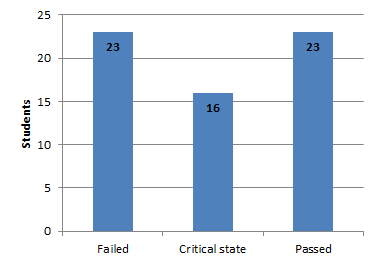
\includegraphics[width=1\linewidth]{img01}
	\caption{Distribution of student's performance}
	\label{fig:DistributionOfStudentPerformance}
\end{figure}
Figure~\ref{fig:DistributionOfStudentPerformance} represents the distribution of student's performance in the experiment, where the evaluation of their submitted code were divided into the three states.\\

As the distribution of the tasks were random, and each student got exactly one task. The number of students receiving the individual tasks were distributed as illustrated in Figure~\ref{fig:TaskDistributions}:

\begin{figure}[!ht]
	\centering
	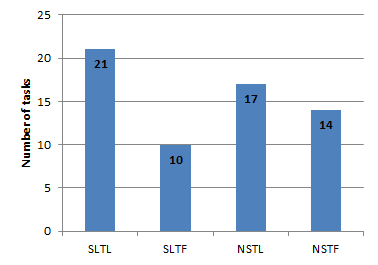
\includegraphics[width=1\linewidth]{img02}
	\caption{Task distributions}
	\label{fig:TaskDistributions}
\end{figure}

38 students used the test-last approach, and 24 students used the test-first approach. Further it is an exceptional case where both the sliced and non-sliced tasks were equally distributed with 31 of each.

After the assessment of the code submissions, it is possible to look at the answers of the questionnaires. Shown in Figure~\ref{fig:Student's own experience rating} the student's perception of their own programming experience in these fields; General programming, C{\#}, Visual Studio, Unit testing, NUnit testing framework and Test-driven development (TDD).
The students were rating their experience on the scale: None, Novice, Intermediate and Expert.

\begin{figure}[!ht]
	\centering
	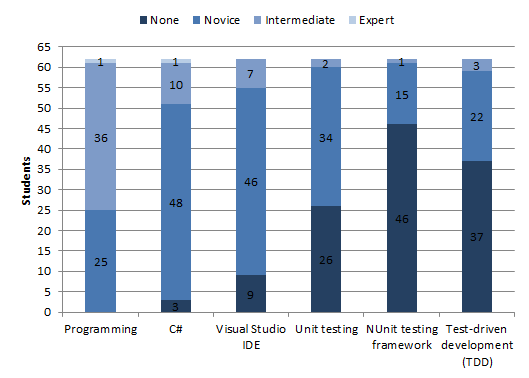
\includegraphics[width=1\linewidth]{img03}
	\caption{Student's own experience rating}
	\label{fig:Student's own experience rating}
\end{figure}

Here is is seen that the students who ended up with TF tasks rated themselves lower in their perception of their experience in TTD.

\begin{figure}[!ht]
	\centering
	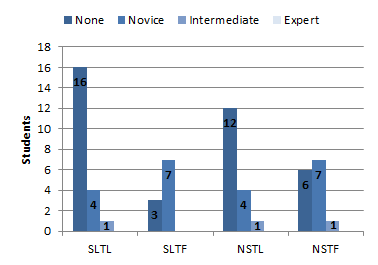
\includegraphics[width=1\linewidth]{img04}
	\caption{TDD experience in tasks}
	\label{fig:TDD experience in tasks}
\end{figure}

When looking at Figure~\ref{fig:Student's own experience rating} and Figure~\ref{fig:TDD experience in tasks}, there are more people with none TDD-experience in the test-last approach, which also is an exceptional case.

The experiment aimed to investigate the performance difference between Test-Driven Development (TDD) and the more common Code First Test After (CFTA) approach, with either step by step instructions (Sliced) or free text (Non-sliced).\\

\subsection{Analysis of data} %lorte overskrift!
As the experiment aimed to investigate the performance based on the four tasks distributed amongst the students, Figure~\ref{fig:Student's task performance} shows the code states divided by the tasks.

\begin{figure}[!ht]
	\centering
	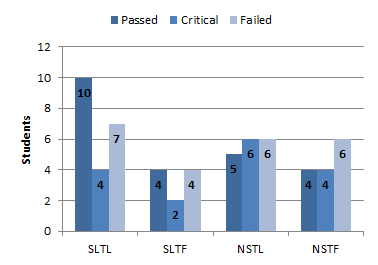
\includegraphics[width=1\linewidth]{img05}
	\caption{Student's task performance}
	\label{fig:Student's task performance}
\end{figure}

As it is stated in Figure~\ref{fig:Student's task performance}, there are a tendency for the students' submissions to pass with sliced tasks.

Figure~\ref{fig:SLTL percentage distributions with relative task numbers} shows the distributions between the students self-rating of programming experience level (None, Novice, Intermediate, Expert), and their correlating submission state (Passed, Critical, Failed), divided into each of the tasks respectively.
It is important to notice that there were no students who have rated their programming experience  as "None" which means that they could have excluded this in Figure~\ref{fig:SLTL percentage distributions with relative task numbers}-\ref{fig:NSTF percentage distributions with relative task numbers}. These are however included in the diagrams as it was an option in the pre-questionnaire, and therefore if excluded, could give a skewed view of the students programming experience levels. This does also apply for the "Expert" ratings which is described show in Figure~\ref{fig:SLTL percentage distributions with relative task numbers}.

\begin{figure}[!ht]
	\centering
	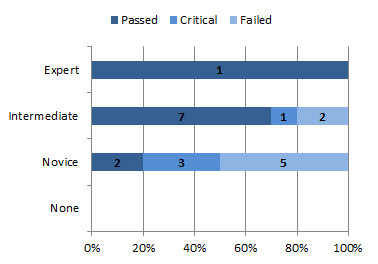
\includegraphics[width=1\linewidth]{img06}
	\caption{Relative distribution and absolute numbers for the SLTL task}
	\label{fig:SLTL percentage distributions with relative task numbers}
\end{figure}

Here it is seen that 100\% of all students who rated their programming experience to be "Expert" has submitted a solution that fulfilled the requirements satisfying, where it was only 70\% and 20\% in respectively "Intermediate" and "Novice".
It is important to notice that there were only one student who rated him- or herself as an "Expert" in programming experience, which means that he could have been excluded from the statistical analysis of this task, as the "Expert" percentage are misleading the reader. The rest of the percentages are for the critical submissions 10\% and 30\%, and for the failed submissions 20\% and 50\% respectively for the "Intermediate" and the "Novice" students.

\begin{figure}[!ht]
	\centering
	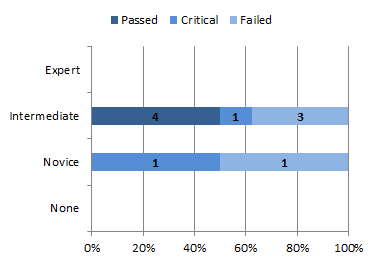
\includegraphics[width=1\linewidth]{img07}
	\caption{Relative distribution and absolute numbers for the SLTF task}
	\label{fig:SLTF percentage distributions with relative task numbers}
\end{figure}

In Figure~\ref{fig:SLTF percentage distributions with relative task numbers} it is seen that only 50\% of the "Inter\-mediate" students submitted solutions which fulfilled the requirements satisfying, where there are none "Novice" students who did. On the other hand it is seen that it is respectively 12.5\% and 50\% in the "Intermediate" and "Novice" who were in the Critical state. The last percentages are 37.5\% and 50\% for respectively the "Intermediate" and the "Novice" students are those who failed.

\begin{figure}[!ht]
	\centering
	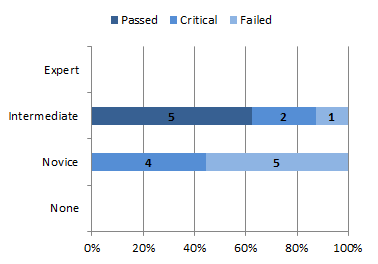
\includegraphics[width=1\linewidth]{img08}
	\caption{Relative distribution and absolute numbers for the NSTL task}
	\label{fig:NSTL percentage distributions with relative task numbers}
\end{figure}

Figure~\ref{fig:NSTL percentage distributions with relative task numbers} shows the distribution of the students' ex\-perience and states of the NSTL tasks. Here it is also seen that it is only the students who have rated themselves as "Inter\-mediate" experienced in programming, who submitted solutions that fulfilled the requirements with 62.5\%. This means that the "Novice" students had a distribution, with 44.5\% critical and 55.5\% failed submissions. Whereas the "Inter\-mediate" students had 25\% critical and 12.5\% failed solution submissions.

\begin{figure}[!ht]
	\centering
	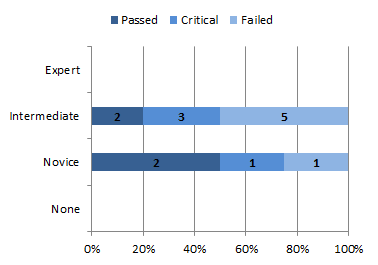
\includegraphics[width=1\linewidth]{img09}
	\caption{Relative distribution and absolute numbers for the NSTF tasks}
	\label{fig:NSTF percentage distributions with relative task numbers}
\end{figure}

Figure~\ref{fig:NSTF percentage distributions with relative task numbers} shows the distribution of the student's experience and states of the NSTF tasks. Here it is seen that both the "Intermediate" and the "Novice" students have submitted solutions that fulfilled the requirements, with a distribution of 20\% and 50\% respectively. Further the critical is distributed 30\% and 25\% where the failed is distributed 50\% and 25\% respectively for the "Intermediate" and the "Novice" students.

Figure~\ref{fig:Total normalized data distributed in tasks} is a visualization of the total normalized data divided into the four different tasks. These data is calculated based on the weights: Passed=1, critical=0.5, failed=0.01. %beskriv beskriv beskriv!n

\begin{figure}[!ht]
	\centering
	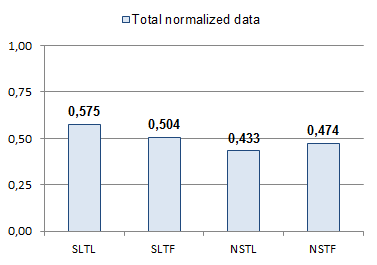
\includegraphics[width=1\linewidth]{img10}
	\caption{Total normalized data distributed in tasks}
	\label{fig:Total normalized data distributed in tasks}
\end{figure}

It is seen that the students who had the sliced tasks performed better than the students who had the non-sliced tasks.

Figure~\ref{fig:Novice normalized data distributed in tasks in accordance to total normalized data} shows "Novice" and "Intermediate" normalized data respectively, in accordance to the total normalized data.

\begin{figure}[!ht]
	\centering
	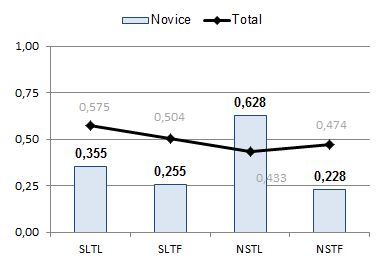
\includegraphics[width=1\linewidth]{img11}
	\caption{Novice normalized data distributed in tasks in accordance to total normalized data}
	\label{fig:Novice normalized data distributed in tasks in accordance to total normalized data}
\end{figure}

In Figure~\ref{fig:Novice normalized data distributed in tasks in accordance to total normalized data} it is illustrated that the "Novice" normalized data is lower than the total in all tasks but in the NSTL task. This data suggest that people who rate their programming experience as "Novice" is more predisposed to doing well when given the NSTL task, than when given one of the other tasks.

\begin{figure}[!ht]
	\centering
	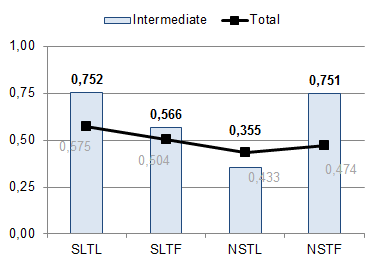
\includegraphics[width=1\linewidth]{img12}
	\caption{Intermediate normalized data ditsributed in tasks in accordance to total normalized data}
	\label{fig:Intermediate normalized data ditsributed in tasks in accordance to total normalized data}
\end{figure}

Figure~\ref{fig:Intermediate normalized data ditsributed in tasks in accordance to total normalized data} shows that the "Intermediate" normalized data is higher than the total in all tasks but in the NSTL. Which suggest that people who rates their programming experience at "Intermediate" is more predisposed to do worse when given the NSTL tasks in comparison if given one of the other tasks.


\section{Discussion}
In this section we compare TDD and CFTA according to our results. The result doesn't give any clear answer to what is best, but the results indicate that for the students as novice developers it was easier to use the code first approach, which could be because they didn't know how to solve the problem at first, but used trial and error to solve small parts of the assignment step by step to find a solution that seemed to cover the requirements. When the developer does not know how the code will be structured in the end it is difficult to write tests that will cover everything.

This has to be compared to the more experienced developers, who knew how they were going to solve the assignment from the requirements. Which allowed them to write the tests according to their initial solution and then use the tests to identify issues they might run into when implementing the logic later on.

But as all of the students are new to programming these are only assumptions, and we have to do more research to find a clear answer, as the results will most likely be different with a group of more experienced developers.

For the next iteration of this experiment it is paramount that the students are more clearly instructed in what the assignment is, to ensure that they are more focused on performing the experiment in accordance to description, as the validity of the results become questionable when the students differ from the described pattern of the experiment. 

To ensure that there was no bias in the assignment of tasks the students received tasks randomly, this has the benefit that we as a group were unable to bias the results by handing out the assignments to the students in a way that would increase the probability of favourable result. The downside to this approach is that there was an unequal distribution of students across the different tasks, but with a sample group of this size it was not an issue.


\section{Threats to validity}
In this section we will go over the threats to validity using the guidelines by Wohlin et al.\cite{wohlin1}.

The threats to the Internal validity of this experiment are mostly related to the selection process. The experiment was conducted while the students were performing a test, which would indicate that they were highly motivated to perform well.

Further External threats to the validity were amongst others the \textit{Interaction of setting and treatment}, as the test subjects were given small simple tasks to complete, which does not represent a real world setting the results from an experiment in the field might vary. \textit{Interaction of history and treatment} is an important factor as the subjects had received lectures in all the topics tested in the experiment a few weeks up to the experiment. The participants were not representative of the target group (Software Developers) which also had an effect on the results, as they were unable to perform at the same level as the level as the target group.

One of the major Social threats was that the students talked about the tasks during the experiment, which was not intended, as this could hamper their individual performance. Another threat to the Social validity comes from the human discomfort from being evaluated\cite{henchy1}, which can have influenced the results. The main \textit{Hypothesis guessing} threat comes from the students recieving five  weeks of TDD lectures just prior to the experiment, this might have impacted the subjects answers more in favor of TDD in the pre- and post questionnaires as they expected us to want them to be in favour of TDD. 

The results might also have been affected by the student's not having the proper prerequisites ready before the experiment, and therefore spent some of the experiment time on preparing their system. This might have had an impact on how much of the assignment they completed, but as stated in the experiment kit, they were not scores on how much of the assignment they handed in, it was focused on how well the handed in code worked as well as how well tested it was.

The principal Conclusion validity is affected by the \textit{heterogeneity of the subjects} was rather large, as the test subjects was still only in the start of their university education, so their previously programming ability still played a major role in their programming proficiency which is also concerning the External validity. Also we do not claim that the results can be generalized for the entire software developer population, as these students were having difficulties solving the basic programming task they had to hand in. 


\section{Conclusion}
In this study we performed an experiment to investigate if there was an increase in productivity when the using TDD instead of CFTA. The test subjects were not representative of the target group of software developers so these findings only reflect how TDD and CFTA compare when used by students. 

But the experiment indicates that for students considering themselves as Novices making the tests first yielded worse results than Test Last. The students considering themselves as intermediate the Test first seemed to yield the best results. But these results has to be tested further to make any generalized conclusion as there is no clear trend in the results.

In the future we would like to perform a similar test on a group which has a closer relation to the actual target group. We would also investigate if it would be possible to use a metric to determine a subject's programming proficiency objectively instead of using the user's opinion. This will hopefully lead to a more general conclusion regarding the performance differences regarding TDD and CFTA.

\bibliographystyle{abbrv}
\bibliography{sigproc}
%To make a new references list use the combination below
% latex bibtex latex latex

\section{Acknowledgments}

First of all, we wants to thank Dr. Marco Kuhrmann for his participation and help in this experiment. Especially for providing the necessary communication with the former of the experiment kit, and the provided tools and data.

We also wants to thank Davide Fucci, Burak Turhan, Markku Oivo from University of Oulu for providing the experiment kit used in this experiment.

Thanks to all students of 3. semester Software Engineering 2016 of University of Southern Denmark for participating in this project.

\end{document}
